\pdfminorversion=4 % for acroread
%\documentclass[aspectratio=169,t,xcolor={usenames,dvipsnames}]{beamer}
\documentclass[aspectratio=169,t,handout,xcolor={usenames,dvipsnames}]{beamer}
\usepackage{../beamerstyle}
\usepackage{dsfont}
\usepackage{bm}
\usepackage[english]{babel}
\usepackage[utf8]{inputenc}
\usepackage{graphicx}
\usepackage{algorithm}
\usepackage[ruled,vlined,algo2e,linesnumbered]{algorithm2e}
%\usepackage[boxed,vlined]{algorithm2e}
\usepackage{hyperref}
\usepackage{booktabs}
\usepackage{mathtools}

\usepackage{amsmath,amssymb}
\usepackage{listings}
\lstset{frame=lines,framesep=3pt,numbers=left,numberblanklines=false,basicstyle=\ttfamily\small}

\usepackage{subfig}
\usepackage{multicol}
%\usepackage{appendixnumberbeamer}
%
\usepackage{tcolorbox}

\usepackage{pgfplots}
\usepackage{tikz}
\usetikzlibrary{trees} 
\usetikzlibrary{shapes.geometric}
\usetikzlibrary{positioning,shapes,shadows,arrows,calc,mindmap}
\usetikzlibrary{positioning,fadings,through}
\usetikzlibrary{decorations.pathreplacing}
\usetikzlibrary{intersections}
\usetikzlibrary{positioning,fit,calc,shadows,backgrounds}
\pgfdeclarelayer{background}
\pgfdeclarelayer{foreground}
\pgfsetlayers{background,main,foreground}
\tikzstyle{activity}=[rectangle, draw=black, rounded corners, text centered, text width=8em]
\tikzstyle{data}=[rectangle, draw=black, text centered, text width=8em]
\tikzstyle{myarrow}=[->, thick, draw=black]

% Define the layers to draw the diagram
\pgfdeclarelayer{background}
\pgfdeclarelayer{foreground}
\pgfsetlayers{background,main,foreground}

%\usepackage{listings}
%\lstset{numbers=left,
%  showstringspaces=false,
%  frame={tb},
%  captionpos=b,
%  lineskip=0pt,
%  basicstyle=\ttfamily,
%%  extendedchars=true,
%  stepnumber=1,
%  numberstyle=\small,
%  xleftmargin=1em,
%  breaklines
%}

 
\definecolor{blue}{RGB}{0, 74, 153}

\usetheme{Boadilla}
%\useinnertheme{rectangles}
\usecolortheme{whale}
\setbeamercolor{alerted text}{fg=blue}
\useoutertheme{infolines}
\setbeamertemplate{navigation symbols}{\vspace{-5pt}} % to lower the logo
\setbeamercolor{date in head/foot}{bg=white} % blue
\setbeamercolor{date in head/foot}{fg=white}
\setbeamercolor{author  in head/foot}{bg=white} %blue
\setbeamercolor{title in head/foot}{bg=white} % blue
\setbeamercolor{title}{fg=white, bg=blue}
\setbeamercolor{block title}{fg=white,bg=blue}
\setbeamercolor{block body}{bg=blue!10}
\setbeamercolor{frametitle}{fg=white, bg=blue}
\setbeamercovered{invisible}

\makeatletter
\setbeamertemplate{footline}
{
  \leavevmode%
  \hbox{%
  \begin{beamercolorbox}[wd=.333333\paperwidth,ht=2.25ex,dp=1ex,center]{author in head/foot}%
%    \usebeamerfont{author in head/foot}\insertshortauthor
  \end{beamercolorbox}%
  \begin{beamercolorbox}[wd=.333333\paperwidth,ht=2.25ex,dp=1ex,center]{title in head/foot}%
    \usebeamerfont{title in head/foot}\insertshorttitle
  \end{beamercolorbox}%
  \begin{beamercolorbox}[wd=.333333\paperwidth,ht=2.25ex,dp=1ex,right]{date in head/foot}%
    \usebeamerfont{date in head/foot}\insertshortdate{}\hspace*{2em}
%    \insertframenumber\hspace*{2ex} 
  \end{beamercolorbox}}%
  \vskip0pt%
}
\makeatother

%\pgfdeclareimage[height=1.2cm]{automl}{images/logos/automl.png}
%\pgfdeclareimage[height=1.2cm]{freiburg}{images/logos/freiburg}

%\logo{\pgfuseimage{freiburg}}

\renewcommand{\comment}[1]{
	\noindent
	%\vspace{0.25cm}
	{\color{red}{\textbf{TODO:} #1}}
	%\vspace{0.25cm}
}
\newcommand{\notefh}[1]{\textcolor{red}{\textbf{FH:} #1}}
\renewcommand{\comment}[1]{}
\newcommand{\hide}[1]{}
\newcommand{\cemph}[2]{\emph{\textcolor{#1}{#2}}}

\newcommand{\lit}[1]{{\footnotesize\color{black!60}[#1]}}

\newcommand{\litw}[1]{{\footnotesize\color{blue!20}[#1]}}


\newcommand{\myframe}[2]{\begin{frame}[c]{#1}#2\end{frame}}
\newcommand{\myframetop}[2]{\begin{frame}{#1}#2\end{frame}}
\newcommand{\myit}[1]{\begin{itemize}#1\end{itemize}}
\newcommand{\myblock}[2]{\begin{block}{#1}#2\end{block}}


\newcommand{\votepurple}[1]{\textcolor{Purple}{$\bigstar$}}
\newcommand{\voteyellow}[1]{\textcolor{Goldenrod}{$\bigstar$}}
\newcommand{\voteblue}[1]{\textcolor{RoyalBlue}{$\bigstar$}}
\newcommand{\votepink}[1]{\textcolor{Pink}{$\bigstar$}}

\newcommand{\diff}{\mathop{}\!\mathrm{d}}
\newcommand{\refstyle}[1]{{\small{\textcolor{gray}{#1}}}}
\newcommand{\hands}[0]{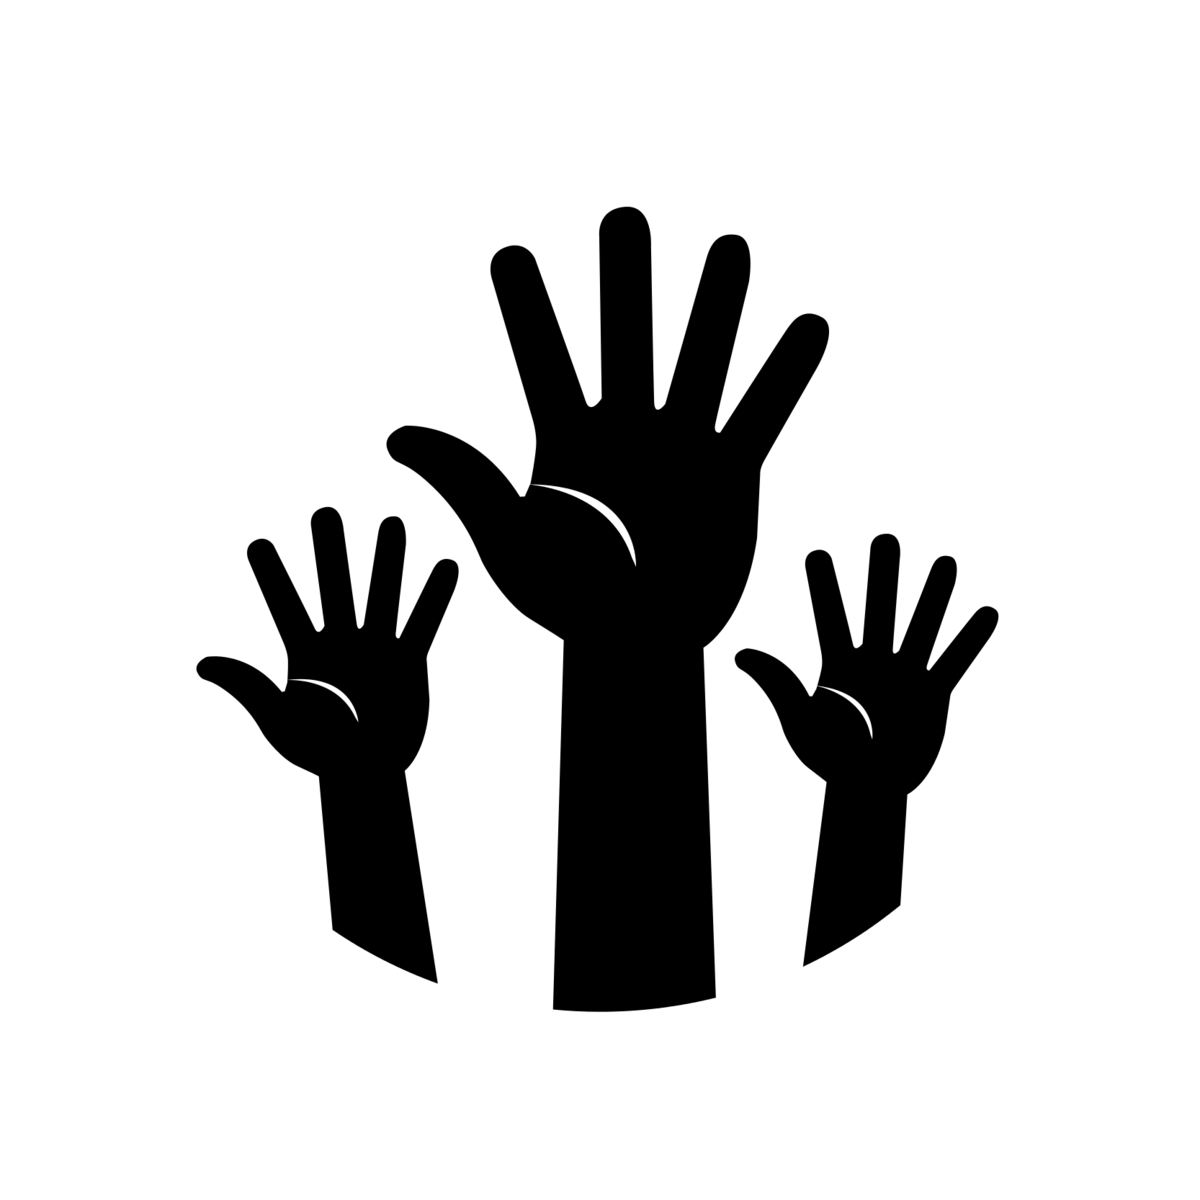
\includegraphics[height=1.5em]{images/hands}}
\newcommand{\transpose}[0]{{\textrm{\tiny{\sf{T}}}}}
\newcommand{\norm}{{\mathcal{N}}}
\newcommand{\cutoff}[0]{\kappa}
\newcommand{\instD}[0]{\dataset}
\newcommand{\insts}[0]{\mathcal{I}}
\newcommand{\inst}[0]{i}
\newcommand{\instI}[1]{i^{(#1)}}

% Iteration specific instance of variable/function/anything
% Introduced in the BO section, but moved up here to make it available within other macros
\newcommand{\iter}[2][\bocount]{{#2}^{(#1)}}

%--------HPO parameter macros-----------

% Parameter Configuration Space
\newcommand{\pcs}[0]{\pmb{\Lambda}}

% ???
\newcommand{\bx}[0]{\conf}

% Parameter Configuration
\newcommand{\conf}[0]{\pmb{\lambda}}

% Final Configuration
\newcommand{\finconf}[0]{\pmb{\hat{\lambda}}}

% Configuration corresponding to a given iteration -- better use \iter!
\newcommand{\confI}[1]{{\conf}^{(#1)}}

% Default Configuration
\newcommand{\defconf}[0]{{\conf}_{\text{def}}}

% Incumbent Configuration
\newcommand{\incumbent}[1][\bocount]{\iter[#1]{\finconf}}

% Optimal Configuration
\newcommand{\optconf}[0]{{\conf}^*}

% Configuration Space
\newcommand{\confs}[0]{\pcs}

%----------------------------------------

%\newcommand{\vlambda}[0]{\bm{\lambda}}
%\newcommand{\vLambda}[0]{\bm{\Lambda}}
\newcommand{\dataset}[0]{\mathcal{D}}
\newcommand{\datasets}[0]{\mathbf{D}}
\newcommand{\loss}[0]{L}
\newcommand{\risk}{\mathcal{R}}
\newcommand{\riske}{\mathcal{R}_{\text{emp}}}
\newcommand{\cost}[0]{c}
\newcommand{\costI}[1]{c^{(#1)}}

% Gaussian Process
\newcommand{\gp}{\mathcal{G}}
% Family of Objective Functions
\newcommand{\objF}{F}

%---------------BO Macros------------------

% BO loop counter
\newcommand{\bocount}{t}
% BO loop counter max, the counter runs from 1 to this value
\newcommand{\bobudget}{T}
% BO loop observation
\newcommand{\obs}[1][\conf]{\cost({#1})}
% BO loop observation space
\newcommand{\obsspace}{\mathcal{Y}}
% BO loop next observation
\newcommand{\bonextobs}{\obs[\iter{\conf}]}
% Acquisition Function, no args
\newcommand{\acq}{u}
% Standard Normal PDF
\newcommand{\pdf}{\phi}
% Standard Normal CDF
\newcommand{\cdf}{\Phi}
% Mean
\newcommand{\mean}{\mu}
% Standard Deviation
\newcommand{\stddev}{\sigma}
% Variance
\newcommand{\variance}{\sigma^2}
% Noise
\newcommand{\noise}{\nu}
% BO loop next selected sample
\newcommand{\bonextsample}{\confI{\bocount}}

% Single hyperparameter
\newcommand{\hyperparam}{\lambda}

% Single hyperparameter within a hyperparameter configuration
\newcommand{\hyperparami}[1][i]{{\hyperparam}_#1}

% Full definition of final configuration
\newcommand{\finconffull}{\incumbent[\bobudget]}

% Dataset
\newcommand{\datasetHPO}{{\dataset}_{HPO}}

% Dataset definition
\newcommand{\datasetHPOdef}{{\langle \bonextsample,\,\bonextobs \rangle}_{\bocount=1}^{\bobudget}}

% Double Display Fraction, forces large displays for everything in numerator and denominator
\newcommand\ddfrac[2]{\frac{\displaystyle #1}{\displaystyle #2}}

% Conditional Probability "Given That" Relation, source:https://tex.stackexchange.com/a/141685/205886
\newcommand\given[1][]{\:#1\vert\:}

% Expectation as a math operator
\DeclareMathOperator*{\E}{\mathbb{E}}

% Citation 
\newcommand{\source}[1]{
    \begin{flushright}
    	Source: \lit{#1}
    \end{flushright}
}
%-------------------------------------------

%Real numbers set
\newcommand{\realnum}{\mathbb{R}}
%Configuration space - do not use
%\newcommand{\configspace}{\Theta}
%Instances - do not use
%\newcommand{\instances}{\mathcal{I}}
%Expected value
\newcommand{\expectation}{\mathbb{E}}
%Kernel
\newcommand{\kernel}{\kappa}
%Constraint function
\newcommand{\constraintf}{c}
%Normal distribution
\newcommand{\normaldist}{\mathcal{N}}

% \renewcommand{\vec}[1]{\mathbf{#1}}
\newcommand{\hist}[0]{\dataset_{\text{Hist}}}
\newcommand{\param}[0]{p}
\newcommand{\algo}[0]{\mathcal{A}}
\newcommand{\algos}[0]{\mathbf{A}}
%\newcommand{\nn}[0]{N}
\newcommand{\feats}[0]{\mathcal{X}_{\text{meta}}}
\newcommand{\feat}[0]{\x_{\text{meta}}}
%\newcommand{\cluster}[0]{\vec{h}}
%\newcommand{\clusters}[0]{\vec{H}}
\newcommand{\perf}[0]{\mathbb{R}}
%\newcommand{\surro}[0]{\mathcal{S}}
\newcommand{\surro}[0]{\hat{\cost}}
\newcommand{\func}[0]{f}
\newcommand{\epm}[0]{\surro}
\newcommand{\portfolio}[0]{\mathbf{P}}
\newcommand{\schedule}[0]{\mathcal{S}}

% Machine Learning
\newcommand{\mdata}[0]{\dataset_{\text{meta}}}
\newcommand{\datasettrain}[0]{\dataset_{\text{train}}}
\newcommand{\datasetval}[0]{\dataset_{\text{val}}}
\newcommand{\datasettest}[0]{\dataset_{\text{test}}}
\newcommand{\x}[0]{\mathbf{x}}
\newcommand{\y}[0]{y}
\newcommand{\xI}[1]{\mathbf{x}^{(#1)}}
\newcommand{\yI}[1]{y^{(#1)}}
\newcommand{\fx}{f(\mathbf{x})}  % f(x), continuous prediction function
\newcommand{\Hspace}{\mathcal{H}} % hypothesis space where f is from
\newcommand{\fh}{\hat{f}}       % f hat, estimated prediction function

% Deep Learning
\newcommand{\weights}[0]{\theta}
\newcommand{\metaweights}[0]{\phi}


% reinforcement learning
\newcommand{\policies}[0]{\mathbf{\Pi}}
\newcommand{\policy}[0]{\pi}
\newcommand{\actionRL}[0]{a}
\newcommand{\stateRL}[0]{s}
\newcommand{\statesRL}[0]{\mathcal{S}}
\newcommand{\rewardRL}[0]{r}
\newcommand{\rewardfuncRL}[0]{\mathcal{R}}

\RestyleAlgo{algoruled}
\DontPrintSemicolon
\LinesNumbered
\SetAlgoVlined
\SetFuncSty{textsc}

\SetKwInOut{Input}{Input}
\SetKwInOut{Output}{Output}
\SetKw{Return}{return}

%\newcommand{\changed}[1]{{\color{red}#1}}

%\newcommand{\citeN}[1]{\citeauthor{#1}~(\citeyear{#1})}

\renewcommand{\vec}[1]{\mathbf{#1}}
\DeclareMathOperator*{\argmin}{arg\,min}
\DeclareMathOperator*{\argmax}{arg\,max}

%\newcommand{\aqme}{\textit{AQME}}
%\newcommand{\aslib}{\textit{ASlib}}
%\newcommand{\llama}{\textit{LLAMA}}
%\newcommand{\satzilla}{\textit{SATzilla}}
%\newcommand{\satzillaY}[1]{\textit{SATzilla'{#1}}}
%\newcommand{\snnap}{\textit{SNNAP}}
%\newcommand{\claspfolioTwo}{\textit{claspfolio~2}}
%\newcommand{\flexfolio}{\textit{FlexFolio}}
%\newcommand{\claspfolioOne}{\textit{claspfolio~1}}
%\newcommand{\isac}{\textit{ISAC}}
%\newcommand{\eisac}{\textit{EISAC}}
%\newcommand{\sss}{\textit{3S}}
%\newcommand{\sunny}{\textit{Sunny}}
%\newcommand{\ssspar}{\textit{3Spar}}
%\newcommand{\cshc}{\textit{CSHC}}
%\newcommand{\cshcpar}{\textit{CSHCpar}}
%\newcommand{\measp}{\textit{ME-ASP}}
%\newcommand{\aspeed}{\textit{aspeed}}
%\newcommand{\autofolio}{\textit{AutoFolio}}
%\newcommand{\cedalion}{\textit{Cedalion}}
\newcommand{\fanova}{\textit{fANOVA}}
\newcommand{\sbs}{\textit{SB}}
\newcommand{\oracle}{\textit{VBS}}

% like approaches
\newcommand{\claspfoliolike}[1]{\texttt{claspfolio-#1-like}}
\newcommand{\satzillalike}[1]{\texttt{SATzilla'#1-like}}
\newcommand{\isaclike}{\texttt{ISAC-like}}
\newcommand{\ssslike}{\texttt{3S-like}}
\newcommand{\measplike}{\texttt{ME-ASP-like}}

\newcommand{\irace}{\textit{I/F-race}}
\newcommand{\gga}{\textit{GGA}}
\newcommand{\smac}{\textit{SMAC}}
\newcommand{\paramils}{\textit{ParamILS}}
\newcommand{\spearmint}{\textit{Spearmint}}
\newcommand{\tpe}{\textit{TPE}}


\usepackage{pifont}
\newcommand{\itarrow}{\mbox{\Pisymbol{pzd}{229}}}
\newcommand{\ithook}{\mbox{\Pisymbol{pzd}{52}}}
\newcommand{\itcross}{\mbox{\Pisymbol{pzd}{56}}}
\newcommand{\ithand}{\mbox{\raisebox{-1pt}{\Pisymbol{pzd}{43}}}}

%\DeclareMathOperator*{\argmax}{arg\,max}

\newcommand{\ie}{{\it{}i.e.\/}}
\newcommand{\eg}{{\it{}e.g.\/}}
\newcommand{\cf}{{\it{}cf.\/}}
\newcommand{\wrt}{\mbox{w.r.t.}}
\newcommand{\vs}{{\it{}vs\/}}
\newcommand{\vsp}{{\it{}vs\/}}
\newcommand{\etc}{{\copyedit{etc.}}}
\newcommand{\etal}{{\it{}et al.\/}}

\newcommand{\pscProc}{{\bf procedure}}
\newcommand{\pscBegin}{{\bf begin}}
\newcommand{\pscEnd}{{\bf end}}
\newcommand{\pscEndIf}{{\bf endif}}
\newcommand{\pscFor}{{\bf for}}
\newcommand{\pscEach}{{\bf each}}
\newcommand{\pscThen}{{\bf then}}
\newcommand{\pscElse}{{\bf else}}
\newcommand{\pscWhile}{{\bf while}}
\newcommand{\pscIf}{{\bf if}}
\newcommand{\pscRepeat}{{\bf repeat}}
\newcommand{\pscUntil}{{\bf until}}
\newcommand{\pscWithProb}{{\bf with probability}}
\newcommand{\pscOtherwise}{{\bf otherwise}}
\newcommand{\pscDo}{{\bf do}}
\newcommand{\pscTo}{{\bf to}}
\newcommand{\pscOr}{{\bf or}}
\newcommand{\pscAnd}{{\bf and}}
\newcommand{\pscNot}{{\bf not}}
\newcommand{\pscFalse}{{\bf false}}
\newcommand{\pscEachElOf}{{\bf each element of}}
\newcommand{\pscReturn}{{\bf return}}

%\newcommand{\param}[1]{{\sl{}#1}}
\newcommand{\var}[1]{{\it{}#1}}
\newcommand{\cond}[1]{{\sf{}#1}}
%\newcommand{\state}[1]{{\sf{}#1}}
%\newcommand{\func}[1]{{\sl{}#1}}
\newcommand{\set}[1]{{\Bbb #1}}
%\newcommand{\inst}[1]{{\tt{}#1}}
\newcommand{\myurl}[1]{{\small\sf #1}}

\newcommand{\Nats}{{\Bbb N}}
\newcommand{\Reals}{{\Bbb R}}
\newcommand{\extset}[2]{\{#1 \; | \; #2\}}

\newcommand{\vbar}{$\,\;|$\hspace*{-1em}\raisebox{-0.3mm}{$\,\;\;|$}}
\newcommand{\vendbar}{\raisebox{+0.4mm}{$\,\;|$}}
\newcommand{\vend}{$\,\:\lfloor$}


\newcommand{\goleft}[2][.7]{\parbox[t]{#1\linewidth}{\strut\raggedright #2\strut}}
\newcommand{\rightimage}[2][.3]{\mbox{}\hfill\raisebox{1em-\height}[0pt][0pt]{\includegraphics[width=#1\linewidth]{#2}}\vspace*{-\baselineskip}}






\title{AutoML: Bayesian Optimization for HPO}
\subtitle{High-Dimensional Bayesian Optimization}
\author[Marius Lindauer]{Bernd Bischl \and \underline{Frank Hutter} \and Lars Kotthoff\newline \and Marius Lindauer \and Joaquin Vanschoren}
\institute{}
\date{}
    
    
    
\begin{document}
\maketitle

%-----------------------------------------------------------------------
\begin{frame}[c]{High-Dimensional Bayesian Optimization: Motivation}

\begin{itemize}
%    \item Bayesian Optimization success stories:
%    \begin{itemize}
%        \item robotics, planning, recommendation, automatic algorithm configuration etc.
%    \end{itemize}
%    \pause
    \item Issue: Standard BO works best on problems of moderate dimensions $d\leq20$
%    \pause
    \begin{itemize}
        \item Standard Gaussian processes do not tend to fit well in high dimensions
        \item Maximizing the acquisition function is also computationally challenging
    \end{itemize}
\medskip
\pause

    \item Possible solutions we will discuss:
    \begin{itemize}
        \item Different models, in particular random forests \lit{\href{https://ml.informatik.uni-freiburg.de/papers/11-LION5-SMAC.pdf}{Hutter et al. 2011}}
        \item Embedding into a low-dimensional space (REMBO) \lit{\href{https://ml.informatik.uni-freiburg.de/papers/16-JAIR-REMBO.pdf}{Wang et al. 2016}}
        \item Additive models \lit{\href{http://proceedings.mlr.press/v37/kandasamy15.pdf}{Kandasamy et al. 2015}}
    \end{itemize}
\end{itemize}


\end{frame}


%----------------------------------------------------------------------

\begin{frame}[c]{Low Effective Dimensionality}

\begin{itemize}
%    \item Good coverage of $\pcs$ is required to ensure that the global optimum is found
%    \item The number of evaluations needed to cover $\pcs$ increases exponentially with dimensionality
    \item Many optimization problems in practice have \alert{low effective dimensionality}
    \begin{itemize}
        \item E.g., HPO for deep neural networks
        \lit{\href{http://www.jmlr.org/papers/volume13/bergstra12a/bergstra12a.pdf}{Bergstra et al. 2012}}
        \item E.g., algorithm configuration for combinatorial optimization solvers \lit{\href{http://www.jmlr.org/papers/volume13/bergstra12a/bergstra12a.pdf}{Hutter et al. 2014}}
    \end{itemize}
\pause
\medskip
    \item \alert{Idea: Exploit low effective dimensionality to cover a lower-dimensional space well}
\end{itemize}

\end{frame}

%----------------------------------------------------------------------

%---------------------------------------------------------------------
\begin{frame}[c]{Using Random Forests for High Dimensions / Low Effective Dimensionality}

    \myit{
        \item Random forests are \alert{automatic feature detectors}
        \myit{
            \item They automatically select the important (axis-aligned) inputs
        }
        \medskip
        \item Random forests have indeed be used effectively on spaces of more than 700 hyperparameters
        \myit{
            \item In terms of computational efficiency, they do not pose a bottleneck
            \item In terms of statistical efficiency, they scale more gracefully to high dimensions than GPs
        }
    }
\end{frame}
%----------------------------------------------------------------------

%----------------------------------------------------------------------
\begin{frame}[c]{Random Embeddings for Exploiting Low Effective Dimensionality: Overview}

Given a $D=2$ dimensional black-box function $\cost(x_{1},x_{2})$:
\begin{itemize}
\begin{columns}[T]
\begin{column}{0.45\linewidth}


    \item Assume we know $\cost$ has only $d=1$ important dimensions, but we don't know which one it is.
    \end{column}
    \begin{column}{0.5\linewidth}
        \begin{figure}
    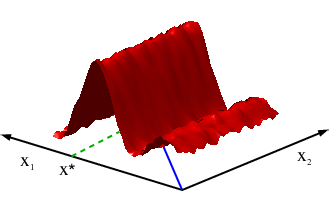
\includegraphics[width=0.5\textwidth]{images/highdim_images/Random_embeddings_in_a_nutshell1.png}
    \end{figure}
    \end{column}
\end{columns}
    \pause
    \begin{columns}[T]
    \begin{column}{0.45\linewidth}
    \vspace{-1em}
    \item Subspace $x_1=x_2$ is guaranteed to include the optimum.
        \end{column}
        \begin{column}{0.5\linewidth}
    \begin{figure}
    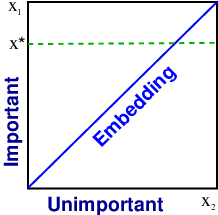
\includegraphics[width=0.5\textwidth]{images/highdim_images/Random_embeddings_in_a_nutshell2.png}
    \end{figure}
    \end{column}
\end{columns}
    \pause
\begin{columns}
\begin{column}{0.45\linewidth}
    \vspace{-8em}
    \item This idea applies to any $d$-dimensional linear subspace; allows scaling to arbitrary $D$ (e.g., $D=1$ billion)
\end{column}
\begin{column}{0.5\linewidth}

\end{column}
\end{columns}
\end{itemize}


\end{frame}

%----------------------------------------------------------------------
\begin{frame}[c]{Random Embedding Bayesian Optimization (REMBO)}
\begin{columns}[T]
\begin{column}{0.01\textwidth}
\end{column}
\begin{column}{0.5\textwidth}
\begin{itemize}
    \item Generate a \alert{random matrix $A \in \realnum^{D \times d}$}
%    \item Choose a bounded region set $\obsspace\subset\realnum^d$
    \item \alert{Use BO to optimize $g(\conf)=\cost(\pmb{Ay})$} instead of high dimensional $\cost(\conf)$
\end{itemize}

\onslide<2->{   
\bigskip
\myblock{Theorem}{
If the effective dimensionality of $c$ is at most d, then with probability 1, for any $\conf\in \realnum^{D}$, there exists a $\pmb{y}\in\realnum^d$ such that $c(\conf) = c(\pmb{Ay})$.}
}
\end{column}
\onslide<1->{
\begin{column}{0.49\textwidth}
\begin{figure}
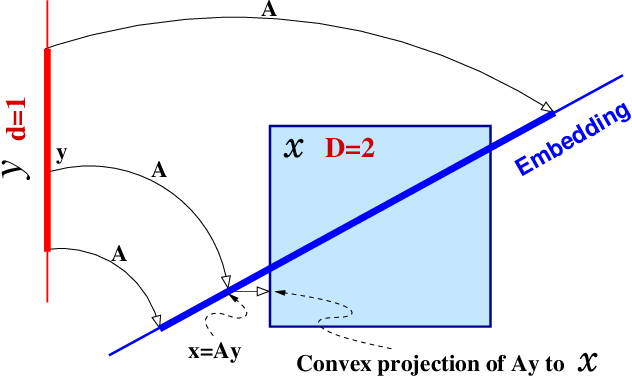
\includegraphics[width=0.8\textwidth]{images/highdim_images/Embedding.png}
\end{figure}
\end{column}
}

\end{columns} 
\end{frame}

%----------------------------------------------------------------------

%----------------------------------------------------------------------
\begin{frame}[c]{High Dimensional Bayesian Optimization: REMBO Pseudocode}

\begin{center}
\begin{minipage}{0.85\textwidth}

\begin{algorithm}[H]
%    \SetAlgoLined
    \setcounter{AlgoLine}{0}
    \SetKwInOut{Require}{Require}
    \SetKwInOut{Result}{Result}
    
    \Require{Search space $\pcs$, cost function $\cost$, acquisition function $\acq$, predictive model $\surro$, maximal number of function evaluations $\bobudget$}
    \Result{Best observed configuration $\finconf$ according to $\iter[\bobudget]{\dataset}$ or $\surro$}
    
    \textcolor{blue}{Generate a random matrix $\pmb{A} \in \realnum^{D\times d}$}\;
    
%    \textcolor{blue}{Choose the bounded region set $\obsspace\subset\realnum^d$}\;
    
    $\iter[0]{\dataset} \leftarrow \varnothing$\; 
	 
    \For{$\bocount=1$ \KwTo $\bobudget$}{
		$\iter[\bocount]{\surro} \leftarrow$ fit predictive model on $\iter[\bocount-1]{\dataset}$\;
		
		\textcolor{blue}{$\pmb{y} \leftarrow \pmb{y} \in \argmax_{\pmb{y}\in\obsspace} \acq(\pmb{y}|\iter[\bocount-1]{\dataset}, \iter[\bocount]{\surro})$}\;
		
		Query $\cost(\textcolor{blue}{\pmb{A}\pmb{y}})$;
		
		$\iter[\bocount]{\dataset} \leftarrow \iter[\bocount-1]{\dataset} \cup \{\langle \textcolor{blue}{\pmb{A}\pmb{y}}, \cost(\textcolor{blue}{\pmb{A}\pmb{y}}) \rangle \}$\;
	}
    \caption*{REMBO: Bayesian Optimization with Random Embedding}
\end{algorithm}

\end{minipage}
\end{center}

\end{frame}
%----------------------------------------------------------------------
\begin{frame}[c]{High Dimensional Bayesian Optimization}
\framesubtitle{Random Embedding Bayesian Optimization - Summary}
\begin{columns}[T] % align columns
\begin{column}{.48\textwidth}


    \begin{block}{Advantages}
    \begin{itemize}
    	\item Exploits low effective dimensionality 
    	\item Allows scaling to arbitrarily high extrinsic dimensions
    	\item Applies to both continuous and categorical variables
    	\item Trivial modification of BO algorithm
    	\item Coordinate independent (invariant under rotations)
    \end{itemize}
    \end{block}
\pause
\end{column}%

\hfill%

\begin{column}{.48\textwidth}

    \begin{block}{Disadvantages}
    \begin{itemize}
    	\item Sensitive to the definition of the bounded low dimensional constrained space $\obsspace$
    	\item Assumes truly unimportant dimensions
    	%Limits a high dimensional function in a low dimensional embedding
    	%\item Sensitive to the effective dimension
    \end{itemize}
\end{block}

\end{column}
\end{columns}   
\end{frame}

%----------------------------------------------------------------------
\begin{frame}[c]{High Dimensional Bayesian Optimization via Additive Models}

\medskip
\begin{itemize}
    \item Recall:

    \begin{itemize}
        \item Standard GPs do not tend to fit well in high dimensions
        \item Maximizing the acquisition function is also computationally challenging
    \end{itemize}
\medskip
\pause
    \item Idea:
    \begin{itemize}
        \item Assume additive structure of the objective function \lit{\href{http://proceedings.mlr.press/v37/kandasamy15.pdf}{Kandasamy et al. 2015}}:
        \begin{equation*}
            \alert{f(\conf)=f^{(1)}(\conf^{(1)})+f^{(2)}(\conf^{(2)})+...+f^{(M)}(\conf^{(M)})}
        \end{equation*}
        \item Model each $f^{(i)}$ by an individual GP
\medskip
\pause
        \item If the decomposition does not overlap:\\
        can maximize acquisition function separately for each of the $f^{(i)}$
\medskip
\pause
        \item Best results for known decomposition, but also possible to learn decomposition from the data
    \end{itemize}
\end{itemize}

\end{frame}

\iffalse
%----------------------------------------------------------------------
\begin{frame}[c]{High Dimensional Bayesian Optimization}
\framesubtitle{Additive GP Models in a nutshell}
        \begin{equation*}
            f(\conf)=f^{(1)}(\conf^{(1)})+f^{(2)}(\conf^{(2)})+...+f^{(M)}(\conf^{(M)})
        \end{equation*}
\begin{itemize}
\begin{columns}[T]
\begin{column}{0.45\linewidth}

\hspace{2em}
    \item Key assumption: $f$ decomposes into lower-dimensional additive components $\conf^{(j)} \in \pcs^{(j)}, j \in \{1,..,M\}$
    \item The decompositions are disjoint $\conf^{(i)} \cap \conf^{(j)} = \varnothing$
    \pause
    \item Each decomposition $f^{(j)}(\conf^{(j)})$ is modelled by an individual GP
    \pause
    \end{column}
    \begin{column}{0.45\linewidth}
        \begin{figure}
    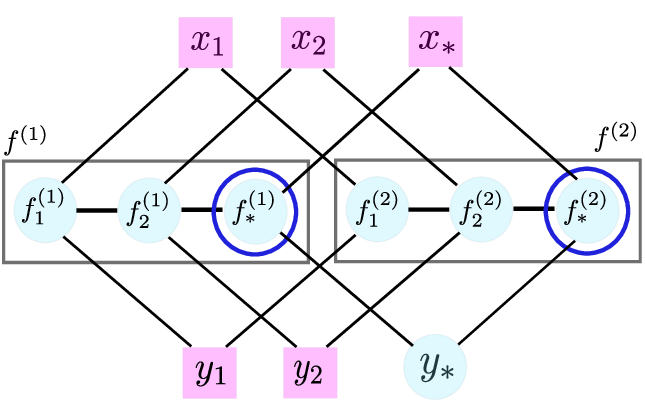
\includegraphics[width=0.7\textwidth]{images/highdim_images/additive-models.png}
    \caption{Decomposition in two additive components (M=2)} 
    \end{figure}
    \end{column}
\end{columns}
\end{itemize}
\end{frame}

%----------------------------------------------------------------------

\begin{frame}[c]{High Dimensional Bayesian Optimization}
\framesubtitle{Additive GP-UCB}
\begin{itemize}

    \item Idea: Represent acquisition function as sum of functions on decompositions:
    \begin{equation*}
        \acq_{t}(\conf) = \sum_{j}\acq_{t}^{(j)}(\conf^{(j)})
    \end{equation*}
\pause
\medskip    
    \item $\acq_{t}$ is maximized by maximizing each $\acq_{t}^{(j)}$ separately:
    \begin{equation*}
        \hat{\varphi}_{t}^{(j)}(\conf^{(j)}) = \mean_{t-1}^{(j)}(\conf^{(j)}) + \beta_{t}^{1/2}\stddev_{t-1}^{(j)}(\conf^{(j)})
    \end{equation*}
    \item Authors have used UCB for this work, but other acquisition functions are possible, too.
\end{itemize}
\source{\href{http://proceedings.mlr.press/v37/kandasamy15.pdf}{Kandasamy et al. 2015}}
\end{frame}
%----------------------------------------------------------------------

\fi
% \begin{frame}[c]{High Dimensional Bayesian Optimization}
% \framesubtitle{Additive GP-UCB- Pseudocode}
% \begin{algorithm}[H]
%     %\DontPrintSemicolon
%     \LinesNumbered
%     \SetAlgoLined
%     \setcounter{AlgoLine}{0}
%     \SetKwInOut{Input}{Input}
    
%     %\Input{Kernels $\kernel^{(1)},...,\kernel^{(M)}$, Decomposition $(\pcs^{(j)})_{j=1}^{M}$}\\
%     \Input{ Kernels $\kernel^{(1)},...,\kernel^{(M)}$, Decomposition $(\pcs^{(j)})_{j=1}^{M}$
%     $\dataset_{0}\leftarrow\varnothing$}
%     \For{$j=1,...,M$, $(\mean_0^{(j)},\kernel_0^{(j)})\leftarrow(0,\kernel^{(j)})$.}{
%         \For{$j=1,...,M$,}{
%             $\confI{t}_{(j)}\leftarrow\argmax_{z\in\pcs^{(j)}}\mean_{t-1}^{(j)}(z) +\sqrt{\beta_{t}}\stddev_{t-1}^{(j)}(z)$;\
            
%             $\confI{t}\leftarrow\bigcup_{j=1}^{M} \confI{t}_{(j)}$;\
            
%             $\obs\leftarrow$ Query $\cost$ at $\confI{t}$;\
            
%             $\dataset_{t}=\dataset_{t-1}\cup\{(\confI{t},\obs)\}$;\
            
%             Perform Bayesian Optimization posterior updates conditioned on $\dataset_{t}$ to obtain $\mean_{t}^{(j)},\stddev_{t}^{(j)}$ for $j=1,...,M$;\
%         }
%     }
%     \caption{Add-GP-UCB}
% \end{algorithm}
% \end{frame}


%----------------------------------------------------------------------
\begin{frame}[c]{High Dimensional Bayesian Optimization via Additive Models}
\begin{columns}[T] % align columns
\begin{column}{.48\textwidth}


    \begin{block}{Advantages}
    \begin{itemize}
    	\item Exploits low effective dimensionality
    	\item Scales GPs to high-dimensional parameter spaces
    	\item Regret is linearly dependent on the dimension D when $\cost$ is additive
%    	\item Add-GP-UCB applies to an additive kernel
    \end{itemize}
    \end{block}
\pause
\end{column}%

\hfill%

\begin{column}{.48\textwidth}

    \begin{block}{Disadvantages}
    \begin{itemize}
    	\item Sensitive to the number of additive components
    	\item Restricted to an axis-aligned representation
        \item Relies on assumption of additivity
        %structural assumptions about the objective function
    \end{itemize}
\end{block}

\end{column}
\end{columns}   
\end{frame}


%%%%%%%%%%%%%%%%%%%%%%%%%%%%%%%%%%%%%%%%%%%%%%%%%%%%%%
\begin{frame}[c]{Questions to Answer for Yourself / Discuss with Friends}

\begin{itemize}

\item \alert{Repetition.} What is the main assumption behind REMBO?
\medskip

\item \alert{Repetition.} What is the main assumption behind additive modelling? 
\medskip

\item \alert{Discussion.} Are these assumptions likely satisfied for tuning deep neural networks?
\medskip

\item \alert{Discussion.} How do random forests help deal with high dimensions and low effective dimensionality? Can they also model additive structure?


\end{itemize}
\end{frame}
\end{document}